\section{ White Noise spectral density}

Let's explore the representation of  White Noise $e(t) \sim WN (\mu,\lambda^2)$, which can be depicted as:
\begin{figure}[H]
    \centering
    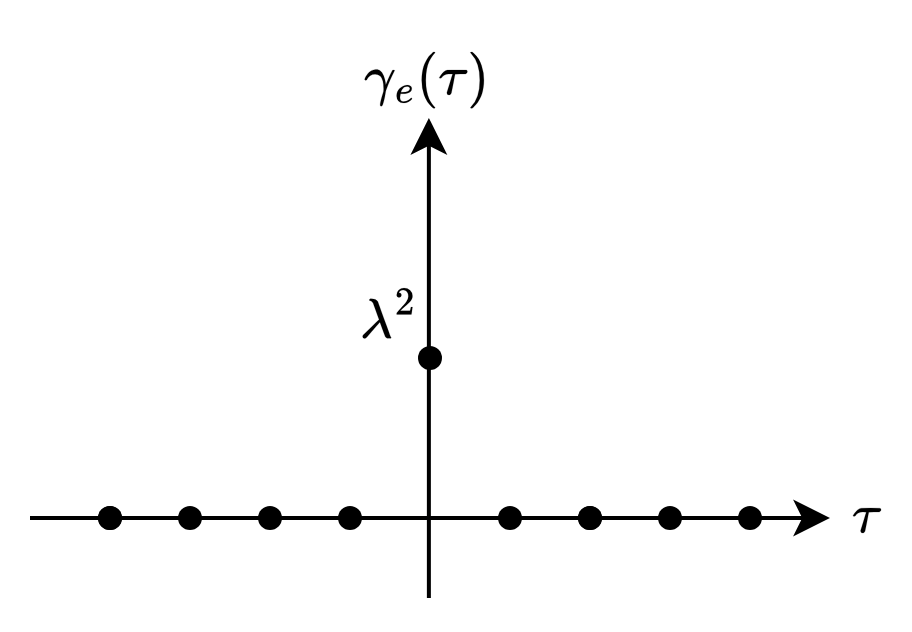
\includegraphics[width=0.35\linewidth]{images/wn1.png}
    \caption{ White Noise covariance function}
\end{figure}

The spectral density of  White Noise is determined as:
\[\Gamma_e(\omega)=\sum_{\tau=-\infty}^{+\infty}\gamma_e(\tau)e^{-j\omega\tau}\]
Since the covariance function $\gamma_e(\tau)$ solely holds a non-zero value at $\tau=0$, the spectral density is essentially the sum of the variance and an infinite series of zeros:
\[\Gamma_e(\omega)=\gamma_e(0)e^{-j\omega 0}+0+\cdots+0=\gamma_e(0)=\lambda^2\]
Here's a visualization of the spectral density function for  White Noise:
\begin{figure}[H]
    \centering
    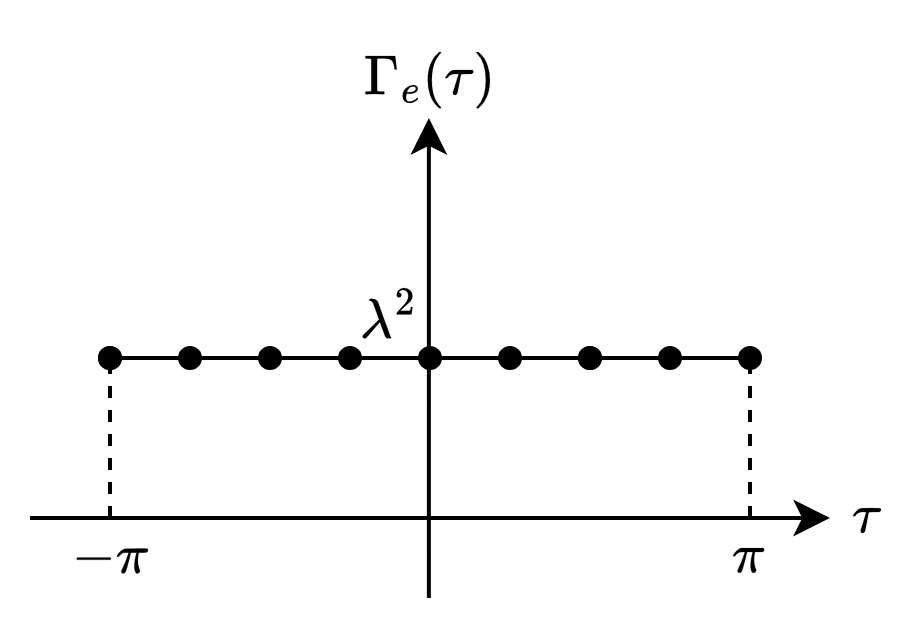
\includegraphics[width=0.35\linewidth]{images/wn2.png}
    \caption{ White Noise spectral density function}
\end{figure}